\documentclass[12pt]{article}
\usepackage[margin=1.2in]{geometry}
\usepackage[all]{nowidow}
\usepackage[hyperfigures=true, hidelinks, pdfhighlight=/N]{hyperref}
\usepackage[separate-uncertainty=true,group-digits=false]{siunitx}
\usepackage{graphicx,amsmath,physics,tabto,float,amssymb,pgfplots,verbatim,tcolorbox}
\usepackage{listings,xcolor,subfig,keyval2e,caption,import}
\numberwithin{equation}{section}
\numberwithin{figure}{section}
\definecolor{stringcolor}{HTML}{C792EA}
\definecolor{codeblue}{HTML}{2162DB}
\definecolor{commentcolor}{HTML}{4A6E46}
\lstdefinestyle{appendix}{
    basicstyle=\ttfamily\footnotesize,commentstyle=\color{commentcolor},keywordstyle=\color{codeblue},
    stringstyle=\color{stringcolor},showstringspaces=false,numbers=left,upquote=true,captionpos=t,
    abovecaptionskip=12pt,belowcaptionskip=12pt,language=Python,breaklines=true,frame=single}
\lstdefinestyle{inline}{
    basicstyle=\ttfamily\footnotesize,commentstyle=\color{commentcolor},keywordstyle=\color{codeblue},
    stringstyle=\color{stringcolor},showstringspaces=false,numbers=left,upquote=true,frame=tb,
    captionpos=b,language=Python}
\renewcommand{\lstlistingname}{Appendix}
\pgfplotsset{compat=1.17}

\title{Waves}
\author{KDSMIL001 \; PHY2004W PHYLAB2}
\date{\textbf{26 October 2020}}

\begin{document}
    \begin{titlepage}
        \maketitle
        \center
        \tableofcontents
    \end{titlepage}
    
    \section{Introduction}\label{sec:Introduction}
    Electromagnetic waves can propagate on a transmission line as well as in free space. One 
    example of such a transmission line is the coaxial cable, most commonly known as the cable 
    that connects a TV set to an aerial. 

    \section{Aim}\label{sec:Aim}
    The standard for propagating electromagnetic (EM) waves is those propagating in a vacuum, 
    the speed of which is well established as $c=\SI{299792458}{\metre/\second}$, but in this 
    experiment we are more interested in the speed of propagation for EM waves in the coaxial 
    cable. We will also determine the characteristic impedance of the cable. 

    \section{Theory}\label{sec:Theory}
    Coaxial cables are a special type of Transmission Line, with an inner and outer conductor 
    separated by some dielectric. These cables have some intrinsic properties, namely a 
    capacitance and inductance per unit length, which are
    \begin{equation*}
        C=\frac{2\pi\epsilon}{\ln(r_{out}/r_{in})}\hspace{20pt}\text{and}\hspace{20pt}L=\frac{\mu}{2\pi}\ln\frac{r_{out}}{r_{in}}
    \end{equation*}
    where we have $\epsilon$ and $\mu$ are the permittivity and permeability of the dielectric 
    in the cable respectively. For our case, we will actually take $\mu=\mu_0=\SI{4\pi e-7}{\henry/\metre}$. 
    Finally $r_{out}$ and $r_{in}$ are the outer and inner radius of the cable, that is the outer 
    radius of the outer and inner conductor respectively. For and EM wave in the cable, the 
    electric and magnetic energy densities are equal, given by 
    \begin{equation*}
        E_E=\frac{1}{2}CV^2\hspace{20pt}\text{and}\hspace{20pt}E_B=\frac{1}{2}LI^2
    \end{equation*}
    where $V$ and $I$ are the the potential and current at a point in the cable. \newline
    \textbf{Exercise 1:} We want to find an expression for the characteristic impedance $Z_0$ 
    of the cable, so we have 
    \begin{align*}
        Z_0&=\frac{V}{I}=\sqrt{\frac{E_E2}{C}}\sqrt{\frac{L}{2E_B}}\\
        E_E&=E_B\\
        \implies Z_0&=\sqrt{\frac{L}{C}}=\sqrt{\frac{\mu}{2\pi}\ln\frac{r_{out}}{r_{in}}\frac{\ln(r_{out}/r_{in})}{2\pi\epsilon}}\\
        &=\frac{1}{2\pi}\sqrt{\frac{\mu}{\epsilon}}\ln\frac{r_{out}}{r_{in}}
    \end{align*}
    Another characteristic of the coaxial cable is that EM waves will propagate through it at 
    a speed 
    \begin{equation}
        v=\frac{c}{\sqrt{\epsilon\mu}}=\frac{c}{n}
        \label{eqn:PropagationSpeedInMedium}
    \end{equation}
    where we call $n$ the refractive index of the dielectric (at the specific frequency of 
    propagation). \newline
    For these cables, if the characteristic impedance changes at some point, the propagation 
    of the wave will be affected, namely the wave will be partially reflected. The reflection 
    coefficient for a purely resistive load $R$ is given by 
    \begin{equation}
        \mathcal{R}=\frac{R-Z_0}{R+Z_0}
        \label{eqn:ReflectionCoefficient}
    \end{equation}
    Note that 
    \textbf{Exercise 2:} We want to show that $\lim_{R\rightarrow\infty} \mathcal{R}=1$:
    \begin{align*}
        \mathcal{R}&=\frac{R-Z_0}{R+Z_0}\\
        \lim_{R\rightarrow\infty} \frac{R-Z_0}{R+Z_0}&=\lim_{R\rightarrow\infty} \frac{1-\frac{Z_0}{R}}{1+\frac{Z_0}{R}}\\
        &=\frac{1-0}{1+0}=1
    \end{align*}
    By measuring the time it takes for reflections of pulses to return to the start of the cable, 
    we will be able to determine the speed of propagation for the waves in the cable with a known 
    length. A similar technique can be used for more extended waves, such as sine waves. \newline
    \newline
    For the pulses we would expect that, depending on the conditions at the end of the cable, 
    we will have different types of reflection. For an open circuit, that is the cable is not 
    connected to anything on the other side, as we have shown in Exercise 2, $\mathcal{R}=1$, so 
    there will be perfect reflection of the pulse. For a short circuit, $R=0$, so we will have 
    $\mathcal{R}=-1$, resulting in a perfectly reflected wave, but with negative voltage.\newline 
    \newline
    For the extended sine wave, we expect to see particular resonant frequencies depending on 
    the length of the cable, resulting in standing waves. Again these frequencies depend on the 
    condition at the end of the cable. For an open circuit, the resonant frequencies will be 
    \begin{equation}
        f_n=n\frac{v}{4L},\;\;\;\; n=1,3,5\dots
        \label{eqn:OpenResonantFrequency}
    \end{equation}
    For a short circuit, we expect 
    \begin{equation}
        f_n=n\frac{v}{2L},\;\;\;\; n=1,2,3\dots 
        \label{eqn:ShortResonantFrequency}
    \end{equation}
    With both of these, we obviously expect a fundamental frequency with harmonics on top of that, 
    hence the multiple nodes. 
    
    \section{Apparatus}\label{sec:Apparatus}
    \begin{itemize}
        \item Signal generator (with duty cycle control).
        \item Oscilloscope.
        \item Digital multimeter.
        \item Coaxial cable of length $\SI{55.845\pm0.005}{\metre}$ with switch to switch termination 
        end between short circuit, open circuit, and variable resistance. 
    \end{itemize}
    We set up the signal generator to feed into the coaxial cable, measuring the voltage at that 
    point with the oscilloscope. 

    \section{Method}\label{sec:Method}
    \subsection{Propagation Speed of the Wave}\label{sec:PropagationSpeedMethod}
    In this section we aimed to determine the speed at which EM waves propagate through the 
    coaxial cable. We did this by two methods. \newline
    \newline
    Firstly we looked at the pulses. We know the length of the cable, so all we needed to do was 
    time how long it took for the pulse to travel from the start of the cable to the end, be 
    reflected, and return to the start. The velocity will simply be given by 
    \begin{equation}
        v=\frac{2L}{\Delta t}
        \label{eqn:PulseVelocity}
    \end{equation}
    To measure measure this $\Delta t$ we set the signal generator to a square wave with the 
    duty cycle to a minimum (20\%), and set the frequency to 1MHz. We measured $\Delta t$ for 
    both the open and short circuit by looking at the oscilloscope. Using these values we 
    could find $v$ for each. \newline
    \newline
    The second method we used to find $v$ was by using \autoref{eqn:OpenResonantFrequency} and 
    \autoref{eqn:ShortResonantFrequency}, varying the frequency of a sine wave supplied by the 
    signal generator to try find the first and second resonant frequencies of both the open and 
    closed circuit. We could then find $v$ for both. 

    \subsection{Characteristic Impedance}\label{sec:CharacteristicImpedanceMethod}
    In this section we aimed to find the characteristic impedance $Z_0$ of the coaxial cable. 
    For this we use the variable resistance setting for the termination end of the cable. We know 
    from \autoref{eqn:ReflectionCoefficient} that $\mathcal{R}=0$ when $R=Z_0$, and we can find 
    this resistance by looking at the oscilloscope for when the reflections vanish completely 
    while varying the resistance. 

    \section{Results}\label{sec:Results}
    \subsection{Propagation Speed of the Wave}\label{sec:PropagationSpeedResults}
    First, the pulses.
    \begin{figure}[H]
        \begin{center}
            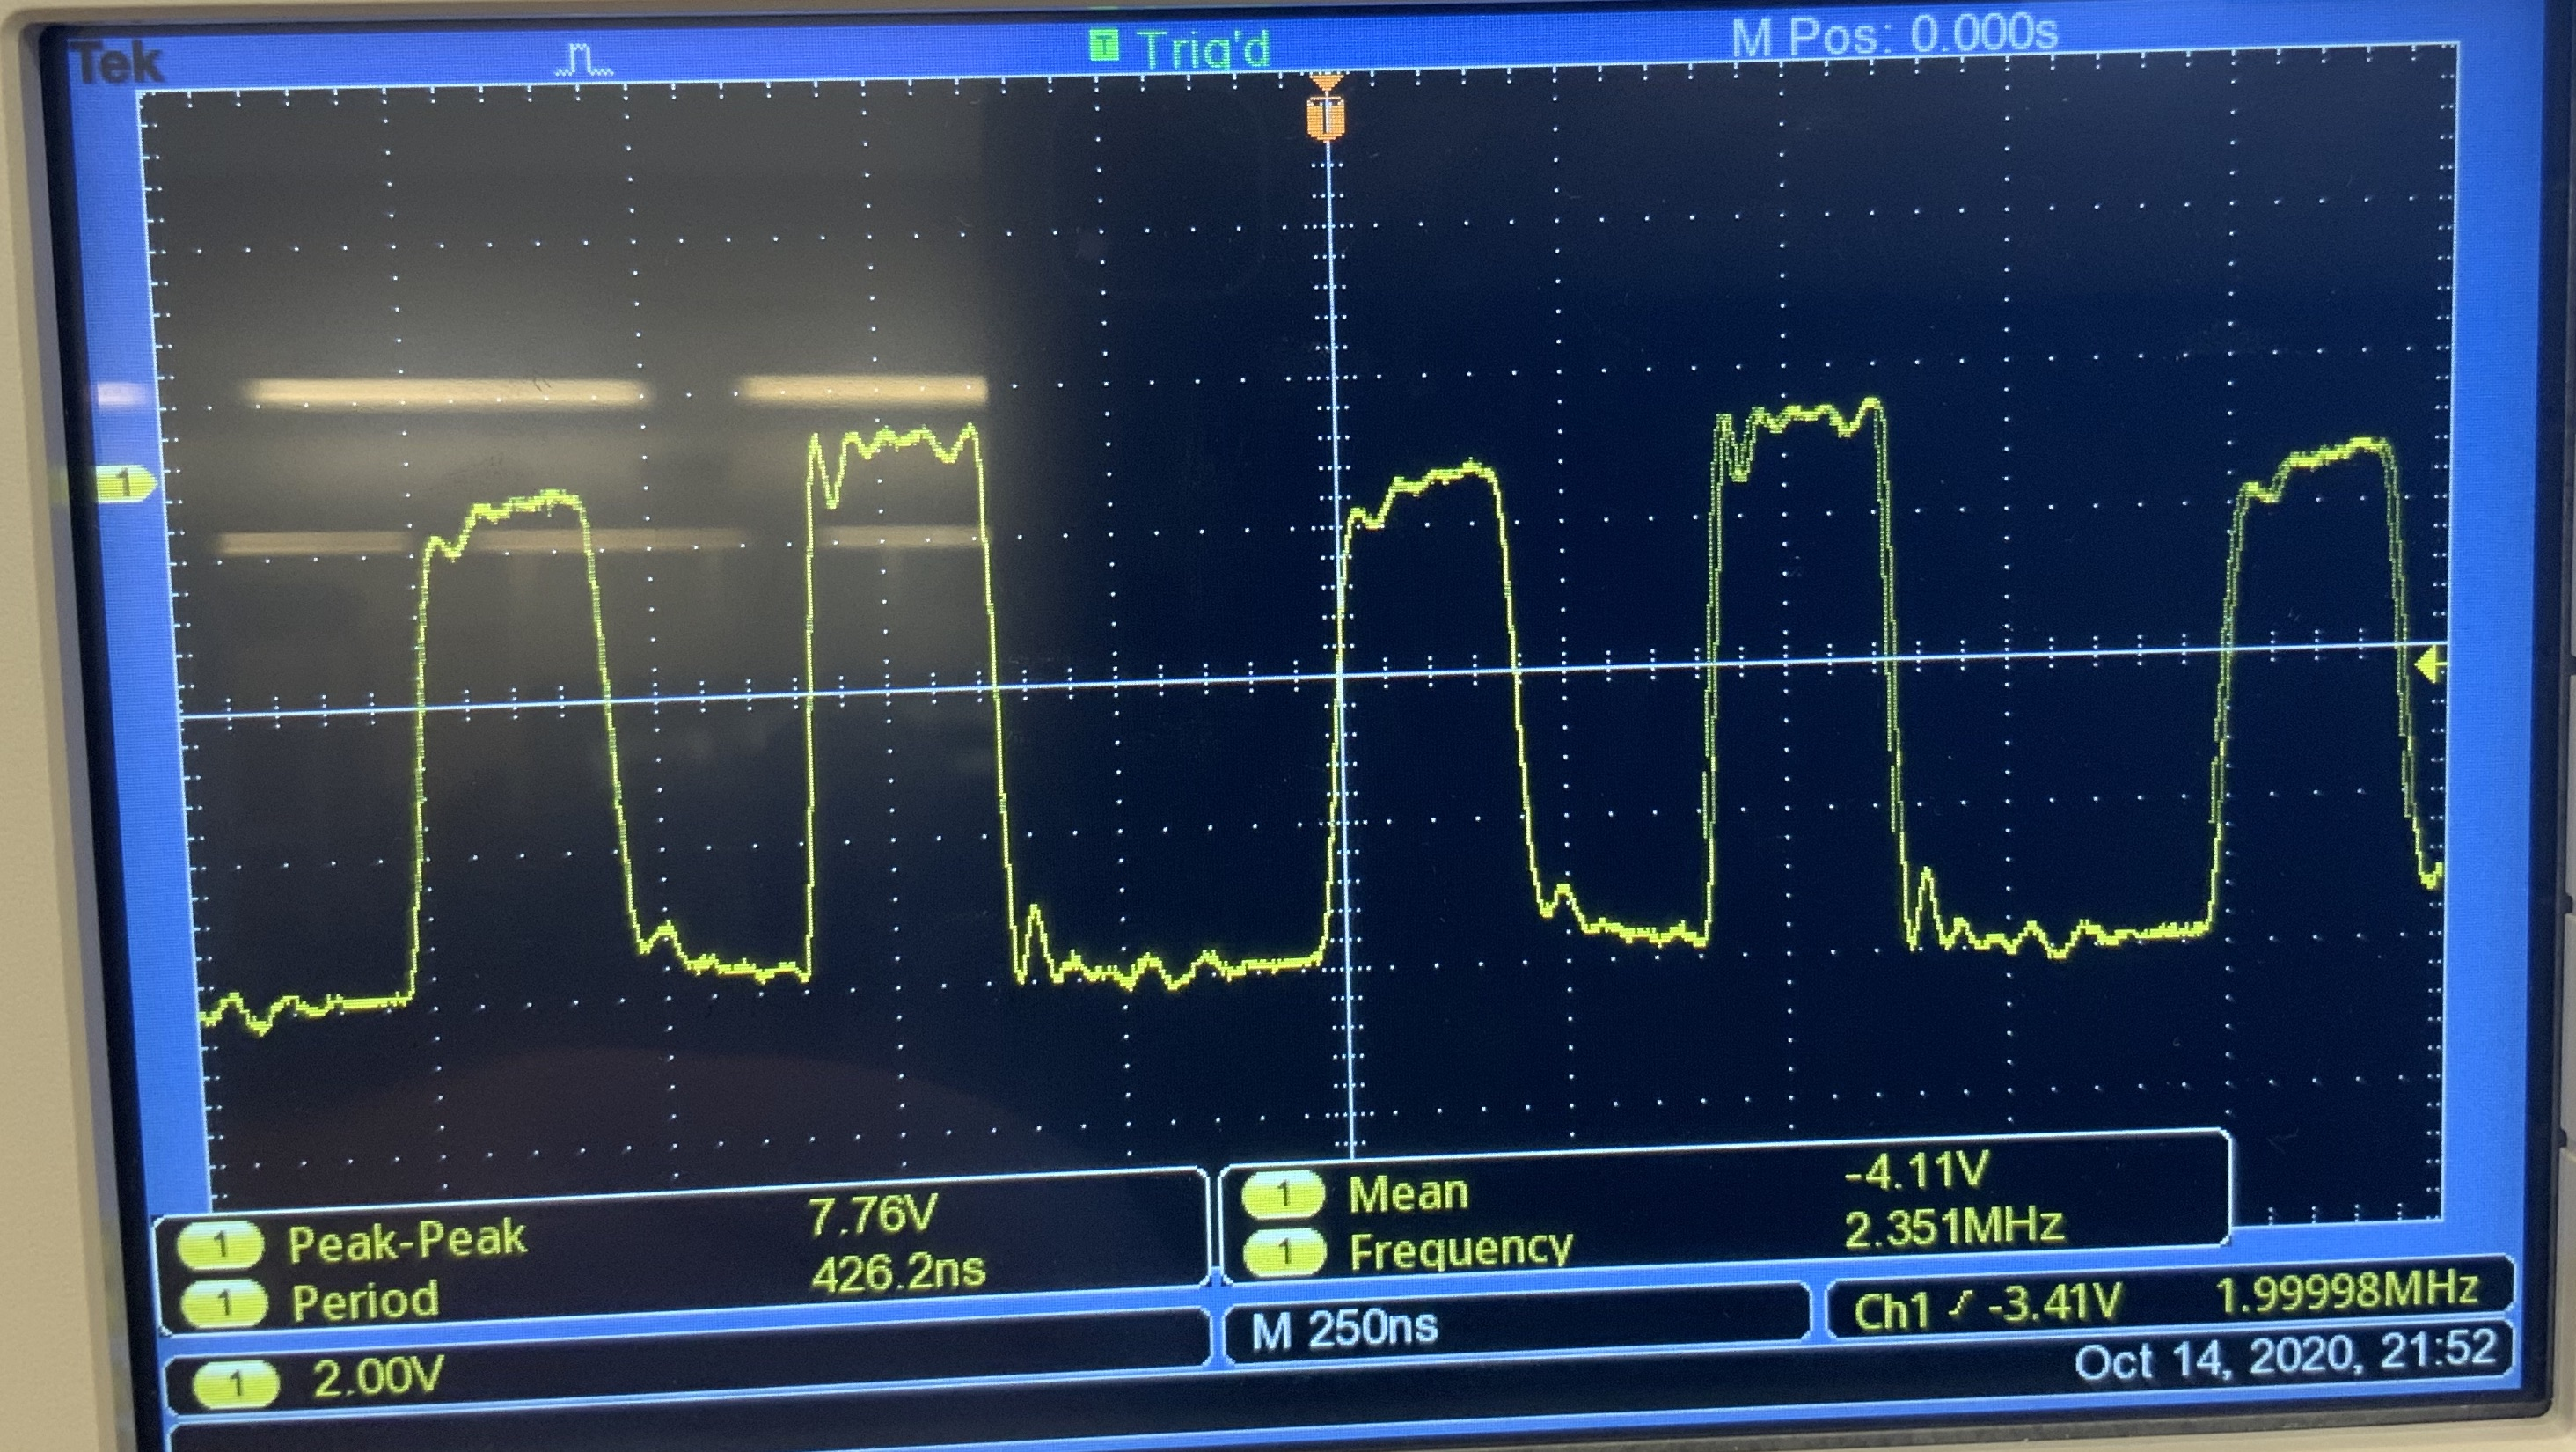
\includegraphics[width=.65\textwidth]{Open_Zoom.jpg}
            \caption{Oscilloscope display showing voltage across the start of an open circuit 
            coaxial cable with 1 MHz square wave signal with duty cycle 20\%.}
            \label{fig:OpenCircuitPulse}
        \end{center}
    \end{figure}
    \begin{figure}[H]
        \begin{center}
            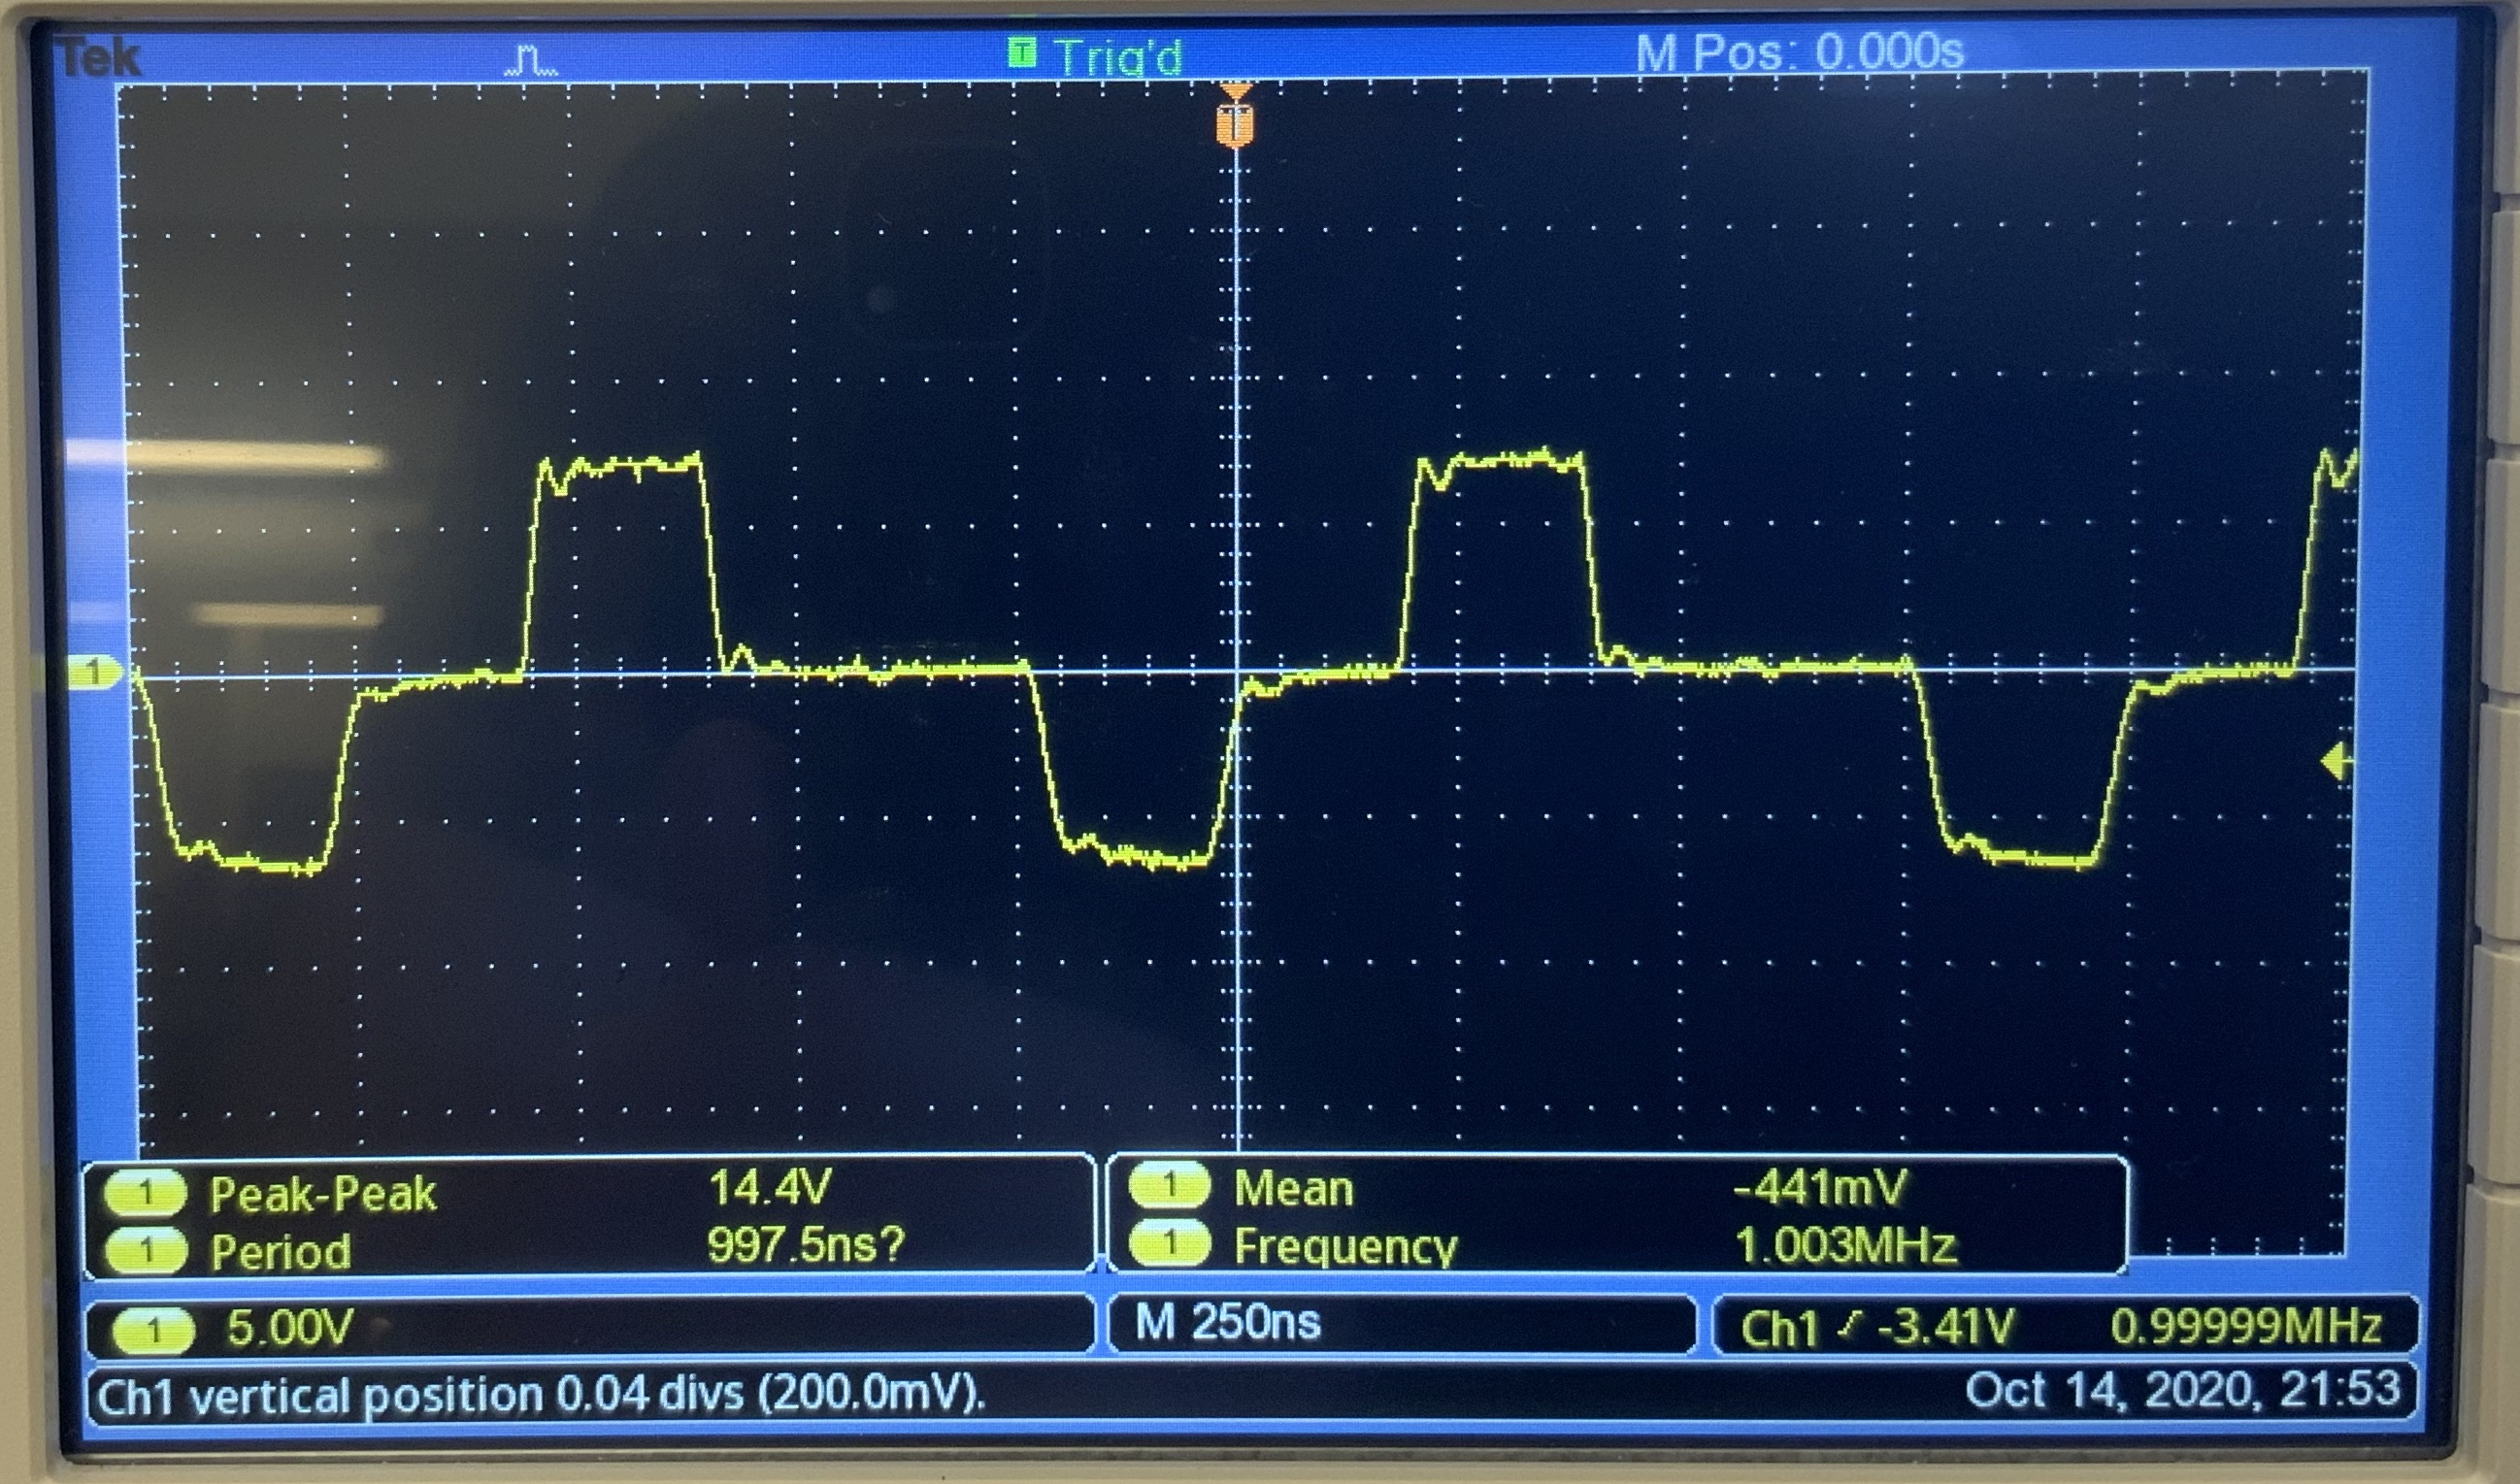
\includegraphics[width=.65\textwidth]{Short_Zoom.jpg}
            \caption{Oscilloscope display showing voltage across the start of a short circuit 
            coaxial cable with 1 MHz square wave signal with duty cycle 20\%.}
            \label{fig:ShortCircuitPulse}
        \end{center}
    \end{figure}
    Measuring from the peak of the first spike of the larger signal to the peak of the first 
    spike of the smaller signal we find a $\Delta t$ of $12\pm1$ small divisions. Looking at the 
    time scale of the oscilloscope we see that each small division is 50 ns. The uncertainty of 
    this measurement comes from 2\% of the time scale, as well as from the triangular pdf 
    associated with analogue measurements. We have, for both the open and short circuits:
    \begin{align*}
        \Delta t&=\SI{600e-9}{\second}\\
        u(\Delta t)&=\sqrt{\left(\frac{2\cdot \num{50e-9}}{2\sqrt{6}}\right)^2 + (0.02\cdot \num{250e-9})^2}\\
        \implies \Delta t&=\SI{600\pm21e-9}{\second}
    \end{align*}
    Using \autoref{eqn:PulseVelocity}, we can find $v$. We have $L=\SI{55.845\pm0.005}{\metre}$ so 
    $2L=\SI{111.69\pm0.01}{\metre}$. The uncertainty comes from the uncertainty propagation for 
    multiplication, giving us
    \begin{align*}
        v&=\frac{111.69}{\num{600e-9}}=\SI{186150000}{\metre\cdot\second^{-1}}\\
        u(v)&=v\sqrt{\left(\frac{u(\Delta t)}{\Delta t}\right)^2 + \left(\frac{u(2L)}{2L}\right)^2}\\
        &=186150000\sqrt{\left(\frac{\num{21e-9}}{\num{600e-9}}\right)^2 + \left(\frac{0.01}{111.69}\right)^2}\\
        &=6515271.317\\
        \implies v_{open}=v_{short}&=\SI{186200000\pm6500000}{\metre\cdot\second^{-1}}
    \end{align*}
    \newline
    Now moving on to the resonant frequencies:
    \begin{table}[H]
        \centering
        \begin{tabular}{c c}
            \textbf{Open} & \\
            \hline
            $f_1$: & $\SI{830\pm1e3}{\hertz}$\\
            $f_3$: & $\SI{2.5\pm0.1e6}{\hertz}$\\
            \hspace{3pt} & \\
            \textbf{Short} & \\
            \hline
            $f_1$: & $\SI{1.7\pm0.1e6}{\hertz}$\\
            $f_2$: & $\SI{3.4\pm0.1e6}{\hertz}$
        \end{tabular}
    \end{table}
    \noindent
    Using these in \autoref{eqn:OpenResonantFrequency} and \autoref{eqn:ShortResonantFrequency}, 
    we find, for the open circuit 
    \begin{align*}
        v_1&=\frac{4f_1L}{1}=185405400\\
        v_3&=\frac{4f_3L}{3}=186150000
    \end{align*}
    and for the short circuit
    \begin{align*}
        v_1&=\frac{2f_1L}{1}=189873000\\
        v_2&=\frac{2f_2L}{2}=189873000
    \end{align*}
    Uncertainty on these values comes from the multiplicative propagation formula, as well as 
    propagation when multiplying by a constant. For the open circuit we find
    \begin{align*}
        u(v_1)&=v_1\sqrt{\left(\frac{u(f_1)}{f_1}\right)^2+\left(\frac{u(L)}{L}\right)^2}\\
        &=223995.9473\\
        u(v_3)&=v_3\sqrt{\left(\frac{u(f_3)}{f_3}\right)^2+\left(\frac{u(L)}{L}\right)^2}\\
        &=7446018.653\\
    \end{align*}
    And for the short circuit:
    \begin{align*}
        u(v_1)&=v_1\sqrt{\left(\frac{u(f_1)}{f_1}\right)^2+\left(\frac{u(L)}{L}\right)^2}\\
        &=11169012.94\\
        u(v_2)&=v_2\sqrt{\left(\frac{u(f_2)}{f_2}\right)^2+\left(\frac{u(L)}{L}\right)^2}\\
        &=5584525.875\\
    \end{align*}
    And so we have 
    \begin{table}[H]
        \centering
        \begin{tabular}{c c}
            \textbf{Open} & \\
            \hline
            $v_1$: & $\SI{185410000\pm220000}{\metre\cdot\second^{-1}}$\\
            $v_3$: & $\SI{186200000\pm7400000}{\metre\cdot\second^{-1}}$\\
            \hspace{3pt} & \\
            \textbf{Short} & \\
            \hline
            $v_1$: & $\SI{189000000\pm11000000}{\metre\cdot\second^{-1}}$\\
            $v_2$: & $\SI{189900000\pm5600000}{\metre\cdot\second^{-1}}$
        \end{tabular}
    \end{table}
    \noindent

    \subsection{Characteristic Impedance}\label{sec:CharacteristicImpedanceResults}
    After finding the frequency which results in having no reflection, we measured it to be 
    \begin{equation*}
        R=\SI{47.1\pm4.0}{\ohm}
    \end{equation*}
    using a digital multimeter. This uncertainty is the uncertainty associated with a digital 
    reading, $\frac{a}{2\sqrt3}$, combined with the 2\% uncertainty rating of the multimeter, 
    which was set to the $200\Omega$ scale. From this we can simply see that 
    \begin{equation*}
        Z_0=\SI{47.1\pm4.0}{\ohm}
    \end{equation*}

    \section{Discussion and Recommendations}\label{sec:DiscussionRecommendations}
    Looking first at the propagation speeds of the EM waves in the coaxial cable, the likely 
    most accurate method would be the first method: measuring the time it takes for a pulse 
    to travel the length of the cable. We say this because the second method requires 
    judgement of the resonant frequency simply by looking at the screen of the oscilloscope as 
    well as tuning the frequency with a signal generator that only increases in relatively 
    large increments. For this reason we will take the first result as being the most accurate 
    and judging the rest off of that one. \newline
    All of the standing wave speeds agree with the pulse speed within their own experimental 
    uncertainty.\newline
    \newline
    Regarding the characteristic impedance of the coaxial cable, we do not have a theoretical 
    estimate for $Z_0$, so we have nothing to compare our value to.

    \section{Conclusion}\label{sec:Conclusion}
    To conclude, we found that we could use two methods to determine the speed of propagation 
    for EM waves in a given coaxial cable and that both of these methods are quite reliable, both 
    supplying values that agree with each other within experimental uncertainty. We also 
    found a value for the characteristic impedance of the coaxial cable, but we could not 
    confirm whether it was a reasonable value.
    
\end{document}